\documentclass[11pt]{article}

\usepackage[a4paper,left=2.5cm,right=2.5cm,top=3.5cm,bottom=3.5cm]{geometry}
\usepackage[utf8]{inputenc}
\usepackage[T1]{fontenc}
\usepackage[english]{babel}
\usepackage{graphicx}
\usepackage{amsmath,amssymb,amsthm,amsopn}
\usepackage{mathrsfs}
\usepackage{graphicx}
\usepackage{array}
\usepackage{makecell}
\usepackage{bm}
\usepackage{hyperref}
\usepackage[shortlabels]{enumitem}
\hypersetup{
    colorlinks=true,
    linkcolor=blue,
    citecolor=red,
}
\usepackage{diagbox}

\usepackage{algorithm}
\usepackage{algpseudocode}

\renewcommand{\algorithmicrequire}{\textbf{Input:}}
\renewcommand{\algorithmicensure}{\textbf{Output:}}

%\usepackage[top=1cm,bottom=1cm]{geometry}
%\usepackage{listings}
%\usepackage{xcolor}

\usepackage{tikz}
\usetikzlibrary{arrows}

% Tikz style

\tikzset{round/.style={circle, draw=black, very thick, scale = 0.7}}
\tikzset{arrow/.style={->, >=latex}}
\tikzset{dashed-arrow/.style={->, >=latex, dashed}}

\newtheoremstyle{break}%
{}{}%
{\itshape}{}%
{\bfseries}{}%  % Note that final punctuation is omitted.
{\newline}{}

\newtheoremstyle{sc}%
{}{}%
{}{}%
{\scshape}{}%  % Note that final punctuation is omitted.
{\newline}{}

\theoremstyle{break}
\newtheorem{thm}{Theorem}[section]
\newtheorem{lm}[thm]{Lemma}
\newtheorem{prop}[thm]{Proposition}
\newtheorem{cor}[thm]{Corollary}

\theoremstyle{sc}
\newtheorem{exo}{Exercice}

\theoremstyle{definition}
\newtheorem{defi}[thm]{Definition}
\newtheorem{ex}[thm]{Example}

\theoremstyle{remark}
\newtheorem{rem}[thm]{Remark}

% Math Operators

\DeclareMathOperator{\Card}{Card}
\DeclareMathOperator{\Gal}{Gal}
\DeclareMathOperator{\Id}{Id}
\DeclareMathOperator{\Img}{Im}
\DeclareMathOperator{\Ker}{Ker}
\DeclareMathOperator{\Minpoly}{Minpoly}
\DeclareMathOperator{\Mod}{mod}
\DeclareMathOperator{\Ord}{Ord}
\DeclareMathOperator{\ppcm}{ppcm}
\DeclareMathOperator{\tr}{Tr}
\DeclareMathOperator{\Vect}{Vect}
\DeclareMathOperator{\Span}{Span}
\DeclareMathOperator{\rank}{rank}
\DeclareMathOperator{\ev}{ev}

% Shortcuts

\newcommand{\dE}{\partial(E)}
\newcommand{\dF}{\partial(F)}
\newcommand{\dG}{\partial(G)}
\newcommand{\diff}{\mathop{}\!\mathrm{d}}
\newcommand{\eg}{\emph{e.g. }}
\newcommand{\emb}{\hookrightarrow}
\newcommand{\embed}[2]{\phi_{#1\hookrightarrow#2}}
\newcommand{\ent}[2]{[\![#1,#2]\!]}
\newcommand{\ie}{\emph{i.e. }}
\newcommand{\ps}[2]{\left\langle#1,#2\right\rangle}
\newcommand{\eqdef}{\overset{\text{def}}{=}}
\newcommand{\f}{f}%{\mathfrak{f}}
\newcommand{\bff}{\mathbf{f}}
\newcommand{\E}{\mathcal{E}}
\newcommand{\A}{\mathcal{A}}
\newcommand{\B}{\mathcal{B}}
\newcommand{\R}{\mathcal{R}}
\newcommand{\bfa}{\mathbf{a}}
\newcommand{\bfb}{\mathbf{b}}
\newcommand{\D}{\mathcal{D}}
\newcommand{\Pcal}{\mathcal{P}}
\newcommand{\musym}{\mu^{\textrm{sym}}}
\newcommand{\mutri}{\mu^{\textrm{tri}}}
\newcommand{\muhyp}{\mu^{\textrm{hyp}}}
\newcommand{\musymG}[1][G]{\mu^{\textrm{sym},#1}}
\newcommand{\mutriG}[1][G]{\mu^{\textrm{tri},#1}}
\newcommand{\muhypG}[1][G]{\mu^{\textrm{hyp},#1}}
\newcommand{\hmusym}{\hat\mu^{\textrm{sym}}}
\newcommand{\hmutri}{\hat\mu^{\textrm{tri}}}
\newcommand{\hmuhyp}{\hat\mu^{\textrm{hyp}}}
\newcommand{\hmusymG}[1][G]{\hat\mu^{\textrm{sym},#1}}
\newcommand{\hmutriG}[1][G]{\hat\mu^{\textrm{tri},#1}}
\newcommand{\hmuhypG}[1][G]{\hat\mu^{\textrm{hyp},#1}}
\newcommand{\Msym}{M^{\textrm{sym}}}
\newcommand{\Mtri}{M^{\textrm{tri}}}
\newcommand{\Mhyp}{M^{\textrm{hyp}}}
\newcommand{\hMsym}{\hat{M}^{\textrm{sym}}}
\newcommand{\hMtri}{\hat{M}^{\textrm{tri}}}
\newcommand{\hMhyp}{\hat{M}^{\textrm{hyp}}}
\newcommand{\tri}[2]{\mu_{#1}^{\text{tri}}(#2)}
\newcommand{\sym}[2]{\mu_{#1}^{m_3}(#2)}
\newcommand{\K}{\mathbf{k}}


% opening
\title{Trisymmetric multiplication formulae in finite fields}
\author{Hugues Randriambololona$^{1, 2}$, Édouard Rousseau$^{2, 3}$}
\date{$^1$ ANSSI, Laboratoire de Cryptographie\\
      $^2$ Institut Polytechnique de Paris, Télécom Paris, LTCI\\
      $^3$ Université Paris-Saclay, UVSQ, CNRS, Laboratoire de Mathématiques de Versailles}

\begin{document}

\maketitle

\begin{abstract}
  Multiplication is an expensive arithmetic operation, therefore there has been
  extensive research to find Karatsuba-like formulae reducing the number of
  multiplications involved when computing a bilinear map. The minimal number of
  multiplications in such formulae is called the \emph{bilinear complexity}, and
  it is also of theoretical interest to asymptotically understand it. Moreover,
  when the bilinear maps admit some kind of invariance, it is also desirable to
  find formulae keeping the same invariance. In this work, we study
  \emph{trisymmetric}, \emph{hypersymmetric}, and \emph{Galois invariant} multiplication formulae over finite fields,
   and we give an algorithm to find such formulae.
  We also generalize the result that the bilinear complexity and symmetric bilinear complexity
  of the
  two-variable multiplication in an extension field are linear in the degree of
  the extension, to trisymmetric bilinear complexity, and to the complexity of $t$-variable
  multiplication for any $t\geq3$.
\end{abstract}

%\tableofcontents
%\clearpage

\section{Introduction}
\label{sec:intro}

%\paragraph{Bilinear complexity.}
Given an algorithm that computes a polynomial map over a field $\K$
(or a family of such polynomial maps, with entries of length going to infinity),
one is
usually interested in the (asymptotic) cost of the algorithm. In order to
understand this cost, one studies the \emph{complexity} of the algorithm, \ie
the number of operations needed by the algorithm. We can for example count the number
of bit operations, or the number of algebraic operations $(+, \times)$ in $\K$. The latter is called the \emph{algebraic complexity}
and in this model it is supposed that all algebraic operations have the same cost.
Nevertheless, multiplication of two variable quantities in $\K$ is arguably more expensive than
addition, or than multiplication of a variable by a fixed constant. In the context of the computation of
bilinear maps, extensive work has been done to reduce the number of
two-variable multiplications involved. Notable examples are Karatsuba's
algorithm~\cite{Karatsuba63} and
Strassen's algorithm~\cite{Strassen69}. Karatsuba's algorithm is
based on the fact that the bilinear map associated to the product of two
polynomials of degree $1$
\[
  A = a_1 X + a_0\text{ and }B = b_1 X + b_0
\]
can be computed with three products $a_0b_0, (a_0+a_1)(b_0+b_1), a_1b_1$ instead
of the four classic ones $a_0b_0, a_0b_1, a_1b_0, a_1b_1$. Strassen's algorithm
exploits a similar idea in the case of $2\times2$ matrices: only $7$ products
are used instead of $8$ in order to compute a matrix product. Both these
algorithms have very practical consequences. The \emph{bilinear complexity}
$\mu(\Phi)$ of a bilinear map $\Phi$ over $\K$ represents the minimum number of two-variable
multiplications in a formula that computes $\Phi$, discarding the cost of other
operations such as addition or multiplication by a constant.
%The bilinear complexity is defined as the minimal number $n$ such that there exist
%linear forms $(\varphi_i)_{1\leq i \leq n}$, $(\psi_i)_{1\leq i \leq n}$ in
%$\A^\vee$, where $\A^\vee$ is the dual of $\A$, and
%elements $(a_i)_{1\leq i \leq n}$ in $\A$ such that
%\begin{equation}
%  \forall x, y\in\A,\,xy = \sum_{i=1}^{n}\varphi_i(x)\psi_i(y)a_i.
%  \label{eq:no-sym}
%\end{equation}
%Equivalently, it can be defined as the rank of the tensor in
%\[
%  \A^\vee \otimes \A^\vee\otimes \A
%\]
%corresponding to the multiplication map in $\A$.
In particular when $\A$ is a finite dimensional algebra over $\K$,
we define the bilinear complexity of $\A$ as $\mu(\A/\K)=\mu(m_{\A})$
where $m_{\A}:\A\times\A\to\A$ is the multiplication map in $\A$ seen
as a $\K$-bilinear map. 

Let $\K^{2\times2}$ be the algebra
of $2\times2$ matrices over $\K$. We know thanks to Strassen's algorithm that 
\[
  \mu(\K^{2\times 2}/\K) \leq 7.
\]
In fact, this is optimal, so we have exactly $\mu(\K^{2\times2}/\K)=7$. In
general, it seems to be hard to find the bilinear complexity of a given algebra,
for example the bilinear complexity of $\K^{3\times3}$ is not known.
In the litterature, work has been done both to algorithmically find the bilinear complexity of
small algebras~\cite{BDEZ12, Covanov19} and to understand how the bilinear
complexity asymptotically grows~\cite{CC88, BCPRRR19}. Chudnovsky and Chudnovsky
proved in 1988 that the bilinear complexity of an extension field
$\mathbb{F}_{q^k}/\mathbb{F}_{q}$ is linear in the degree $k$ of the
extension, using an evaluation-interpolation method on curves.
As the main contribution of this article, we
investigate both questions for \emph{trisymmetric} bilinear complexity,
and solve a certain number of the open problems stated in \cite[\S5.2]{BCPRRR19}.

When a bilinear map admits certain invariance properties, it can be interesting,
both for theoretical and for practical reasons,
to find formulae for it that exhibit these same invariances.
For symmetric bilinear maps, and in particular for commutative algebras, this leads to the notion of symmetric bilinear complexity.
A further refinement, the trisymmetric bilinear complexity of $\mathbb{F}_{q^k}$ over $\mathbb{F}_{q}$, was first introduced in \cite{SL84}, and rediscovered independently in \cite[App.~A]{Randriam15}.

In Section~\ref{sec:symtrisym} we recall the definition of symmetric and trisymmetric formulae, and discuss further generalizations such as hypersymmetric formulae for higher multilinear maps,
and Galois-invariant formulae. In Section~\ref{sec:algos} we
describe algorithms to compute trisymmetric decompositions in small dimension.
In all examples we were able to compute, the trisymmetric bilinear complexity is equal to the symmetric bilinear
complexity. However we found an example where the Galois-invariant trisymmetric bilinear complexity is strictly larger.
Finally, in
Section~\ref{sec:asymptotic}, we prove that for all $q\geq3$, the trisymmetric bilinear
complexity of an extension of $\mathbb{F}_q$ is again linear in the degree, as well as similar results
for higher multiplication maps.

\section{Multiplication formulae with symmetries}
\label{sec:symtrisym}

Although we are mainly interested in bilinear multiplication formulae,
the notions we will consider naturally involve higher multilinear maps.

\paragraph{Multilinear complexity.}
Let $\Phi:V_1\times\cdots\times V_t\to W$
be a $t$-multilinear map between finite dimensional vector spaces over $\K$.
A \emph{multilinear algorithm}, or \emph{multilinear decomposition}, or
\emph{multilinear formula} of length $n$ for $\Phi$ is a collection of linear
forms $(\phi_i^{(j)})_{\substack{1\leq i \leq n\\1\leq j\leq t}}$,
where $\phi_i^{(j)}$ is in $V_j^\vee$, the dual vector space of $V_j$,
and elements $(w_i)_{1\leq i \leq n}$ in $W$, 
such that for all $v_1,\dots,v_t$ we have
\[
  \Phi(v_1,\dots,v_t)=\sum_{i=1}^{n}\varphi_i^{(1)}(v_1)\cdots\varphi_i^{(t)}(v_t)w_i.
\]
The \emph{multilinear complexity} $\mu(\Phi)$ is then defined as the smallest
length $n$ of such a decomposition.
Equivalently, it is the rank of the tensor in
$V_1^\vee \otimes\dots\otimes V_t^\vee\otimes W$
corresponding to $\Phi$.

\paragraph{Symmetric multilinear complexity.}
When $V_1=\cdots=V_t=V$ and $\Phi$ is a \emph{symmetric} multilinear map, it is
natural to search for \emph{symmetric multilinear decompositions}, \ie formulae of the form
\begin{equation*}
  \Phi(v_1,\dots,v_t)=\sum_{i=1}^{n}\varphi_i(v_1)\cdots\varphi_i(v_t)w_i
%  \label{eq:sym}
\end{equation*}
with $\varphi_i^{(1)}=\dots=\varphi_i^{(t)}=\varphi_i\in V^\vee$ for all $i$.
It is more space-efficient, since symmetric formulae admit a shorter description.
On an algorithmic point of view, it should also be simpler to find symmetric formulae,
because the search space is smaller. 
We define $\musym(\Phi)$,
the \emph{symmetric multilinear complexity} of $\Phi$,
as the minimal length $n$ of such a symmetric decomposition, if it exists
(otherwise we set $\musym(\Phi)=\infty$).

In the case $t=2$, a symmetric bilinear map always admits a symmetric decomposition.
However, when $t\geq3$ and $\K=\mathbb{F}_q$ is a finite field, this can fail.
When $t=3$ and $q>2$, it is shown in \cite[Lemma~7]{SL84} that a symmetric trilinear map $\Phi$ over $\mathbb{F}_q$ always admits a symmetric algorithm,
while in the remaining case $t=3$ and $q=2$, as observed by Cascudo,
a necessary condition is that $\Phi$ should satisfy $\Phi(x,x,y)=\Phi(x,y,y)$
for all entries $x,y$.
These results were then combined and generalized into the following necessary and sufficient criterion:
\begin{thm}[{\cite[Thm.~A.7]{Randriam15}}]\label{th:criterion}
Let $\Phi:V^t\to W$ be a $t$-multilinear map between finite dimensional vector spaces over $\mathbb{F}_q$.
Then $\Phi$ admits a symmetric decomposition if and only if $\Phi$ is \emph{Frobenius-symmetric},
\ie if and only if it is symmetric and one of the following two conditions holds:
\begin{itemize}
\item $t\leq q$
\item $t\geq q+1$ and for all $u,v,z_1,\dots,z_{t-q-1}$ in $V$,
\[
\Phi(\underset{\textrm{$q$ times}}{\underbrace{u,\dots,u}},v,z_1,\dots,z_{t-q-1})=\Phi(u,\underset{\textrm{$q$ times}}{\underbrace{v,\dots,v}},z_1,\dots,z_{t-q-1}).
\]
\end{itemize}
\end{thm}
Observe that this criterion involves the \emph{cardinality} of the field, not its characteristic.

\paragraph{Trisymmetric and hypersymmetric complexity.}
Now suppose furthermore that $V=W$, and that this space is equipped with a
non-degenerate symmetric bilinear form, written as a scalar product
\[
\begin{array}{ccc}
V\times V &\to&\K\\
(v,w)&\mapsto&\ps{v}{w}.
\end{array}
\]
This allows to identify $V$ and $V^\vee$, \ie any linear form $\phi\in V^\vee$
is of the form $\phi(x)=\ps{a}{x}$ for a uniquely determined $a\in V$.
As a consequence, a symmetric decomposition for $\Phi:V^t\to V$ can also be described
as the data of elements $(a_i)_{1\leq i\leq n}$ and $(b_i)_{1\leq i\leq n}$ in $V$
such that for all $v_1,\dots,v_t$ in $V$,
we have $\Phi(v_1,\dots,v_t)=\sum_{i=1}^{n}\ps{a_i}{v_1}\cdots\ps{a_i}{v_t}b_i$.
In order to have an even more compact description, one could ask for $b_i$ to be proportional to $a_i$, leading to the following:
\begin{defi}
Let $V$ be a finite dimensional $\K$-vector space equipped with a scalar product,
and $\Phi:V^t\to V$ a symmetric $t$-multilinear map.
Then a \emph{hypersymmetric} formula for $\Phi$ is the data of
elements $(a_i)_{1\leq i\leq n}$ in $V$ and scalars $(\lambda_i)_{1\leq i\leq n}$ in $\K$ such that, for all $v_1,\dots,v_t\in V$,
\[
\Phi(v_1,\dots,v_t)=\sum_{i=1}^{n}\lambda_i\ps{a_i}{v_1}\cdots\ps{a_i}{v_t}a_i.
\]
The hypersymmetric complexity $\muhyp(\Phi)$ is then the minimal length $n$ of such a hypersymmetric decomposition, if it exists. Obviously we always have $\musym(\Phi)\leq\muhyp(\Phi)$.

When $t=2$, we will say \emph{trisymmetric} for hypersymmetric,
and write $\mutri(\Phi)$ for $\muhyp(\Phi)$.
\end{defi}
As a further motivation, observe that to any $t$-multilinear map $\Phi:V^t\to V$
one can associate a $(t+1)$-multilinear \emph{form} $\widetilde{\Phi}:V^{t+1}\to \K$, defined by
\[
\widetilde{\Phi}(v_1,\dots,v_t,v_{t+1})=\ps{\Phi(v_1,\dots,v_t)}{v_{t+1}}.
\]
We then say that $\Phi$ is hypersymmetric (as a $t$-multilinear map)
if $\widetilde{\Phi}$ is symmetric (as a $(t+1)$-multilinear form).
It is easily seen that $\Phi$ hypersymmetric is a necessary condition for it to admit a hypersymmetric decomposition, and more precisely:
\begin{lm}
\label{lm:hyp=symtilde}
Elements $(a_i)_{1\leq i\leq n}$ in $V$ and scalars $(\lambda_i)_{1\leq i\leq n}$ in $\K$ define a hypersymmetric formula for the $t$-multilinear map $\Phi$,
\[
\Phi(v_1,\dots,v_t)=\sum_{i=1}^{n}\lambda_i\ps{a_i}{v_1}\cdots\ps{a_i}{v_t}a_i,
\]
if and only if they define a symmetric formula for the $(t+1)$-multilinear form $\widetilde{\Phi}$,
\[
\widetilde{\Phi}(v_1,\dots,v_s,v_{t+1})=\sum_{i=1}^{n}\lambda_i\ps{a_i}{v_1}\cdots\ps{a_i}{v_t}\ps{a_i}{v_{t+1}}.
\]

Thus, $\Phi$ admits a hypersymmetric formula if and only if $\widetilde{\Phi}$ is Frobenius-symmetric (in the sense of Theorem~\ref{th:criterion}),
and we have
\[
\muhyp(\Phi)=\musym\left(\widetilde{\Phi}\right).
\]

In particular, if $q\geq t+1$, then any hypersymmetric $t$-multilinear map over $\mathbb{F}_q$ admits a hypersymmetric formula.
\end{lm}
\begin{proof}
For the \emph{only if} part in the first assertion, take scalar product with $v_{t+1}$. For the \emph{if} part, use the fact that the scalar product is non-degenerate. The other assertions follow.
\end{proof}

\paragraph{Galois invariance.}
Last we consider another type of symmetry.
Let $\sigma:v\mapsto v^\sigma$ be a $\K$-linear automorphism of $V$
that respects the scalar product: $\ps{v^\sigma}{w^\sigma}=\ps{v}{w}$ for all $v,w$ in $V$.
\begin{lm}
\label{lm:symGalois}
Let $\Phi:V^t\to V$ be a symmetric $t$-multilinear map that is compatible with $\sigma$, \ie
\[
\Phi(v_1^\sigma,\dots,v_t^\sigma)=\Phi(v_1,\dots,v_t)^\sigma
\]
for all $v_1,\dots,v_t$ in $V$,
and let $(a_i)_{1\leq i\leq n}$ and $(b_i)_{1\leq i\leq n}$ in $V$ define a symmetric formula for $\Phi$,
\[
\Phi(v_1,\dots,v_t)=\sum_{i=1}^{n}\ps{a_i}{v_1}\cdots\ps{a_i}{v_t}b_i.
\]
Then $(a_i^\sigma)_{1\leq i\leq n}$ and $(b_i^\sigma)_{1\leq i\leq n}$ also define a symmetric formula for $\Phi$,
\[
\Phi(v_1,\dots,v_t)=\sum_{i=1}^{n}\ps{a_i^\sigma}{v_1}\cdots\ps{a_i^\sigma}{v_t}b_i^\sigma.
\]
\end{lm}
\begin{proof}
Write $\Phi(v_1,\dots,v_t)=\Phi(v_1^{\sigma^{-1}},\dots,v_t^{\sigma^{-1}})^\sigma$ and apply the formula.
\end{proof}
We then say that the symmetric formula given by $(a_i)_{1\leq i\leq n}$ and $(b_i)_{1\leq i\leq n}$ is $\sigma$-invariant if it is the same as the formula given by $(a_i^\sigma)_{1\leq i\leq n}$ and $(b_i^\sigma)_{1\leq i\leq n}$,
\ie if there is a permutation $\pi$ of $\{1,\dots,n\}$ such that $(a_i^\sigma,b_i^\sigma)=(a_{\pi(i)},b_{\pi(i)})$ for all $i$. This applies also to hypersymmetric formulae, setting $b_i=\lambda_i a_i$.

If $G$ is a group of $\K$-linear automorphisms of $V$
that respect the scalar product, and if $\Phi:V^t\to V$ is a symmetric $t$-multilinear map that is compatible with all elements in $G$,
we then define $\musymG(\Phi)$ (resp. $\muhypG(\Phi)$),
the \emph{$G$-invariant} symmetric (resp. hypersymmetric) multilinear complexity of $\Phi$,
as the minimal length $n$ of a symmetric (resp. hypersymmetric) multilinear formula for $\Phi$ that is $G$-invariant, \ie $\sigma$-invariant for all $\sigma$ in $G$. 


\paragraph{Multiplication formulae in algebras}

Let $\A$ be a finite dimensional commutative algebra over $\K$.
We say a linear form $\tau:\A\to\K$ is trace-like if the symmetric bilinear form $\A\times\A\to\K$, $(x,y)\mapsto\tau(xy)$ is non-degenerate.
If so, we set $\ps{x}{y}=\tau(xy)$, which defines a scalar product on $\A$.
In this work we will take $\K=\mathbb{F}_q$, and either:
\begin{itemize}
\item $\A=\mathbb{F}_{q^k}$ a finite field extension, and $\tau=\tr_{\mathbb{F}_{q^k}/\mathbb{F}_q}$ the usual trace map; indeed it is well known that the trace bilinear form $\ps{x}{y}=\tr_{\mathbb{F}_{q^k}/\mathbb{F}_q}(xy)$ is non-degenerate
\item $\A=\mathbb{F}_q[T]/(T^k)$ an algebra of truncated polynomials,
and $\tau$ defined by $\tau(x)=x_{k-1}$ for $x=x_0+x_1T+\dots+x_{k-1}T^{k-1}$ in $\A$;
indeed, observe that for $x=x_0+x_1T+\dots+x_{k-1}T^{k-1}$, $y=y_0+y_1T+\dots+y_{k-1}T^{k-1}$,
we then have $\ps{x}{y}=\tau(xy)=x_0y_{k-1}+x_1y_{k-2}+\dots+x_{k-1}y_0$, which is non-degenerate.
\end{itemize}
Let $\Phi:\A\times\A\to\A$ be the multiplication map, $\Phi(x,y)=xy$.
It is easily seen that $\Phi$ is trisymmetric.
Indeed $\widetilde{\Phi}$ is the trilinear form $x,y,z\mapsto \tau(xyz)$,
which is symmetric.
A symmetric bilinear multiplication formula for $\A$ is thus the data
of $(a_i)_{1\leq i\leq n}$ in $\A$ and $(\varphi_i)_{1\leq i\leq n}$ in $\A^\vee$ such that
\begin{equation}
\forall x, y\in\A,\;xy = \sum_{i=1}^{n}\varphi_i(x)\varphi_i(y)a_i,
\label{eq:sym-tr}
\end{equation}
and a trisymmetric formula is the data of $(a_i)_{1\leq i\leq n}$ in $\A$
and $(\lambda_i)_{1\leq i\leq n}$ in $\mathbb{F}_q$ such that
\begin{equation}
\forall x, y\in\A,\;xy = \sum_{i=1}^{n}\lambda_i\ps{a_i}{x}\ps{a_i}{y}a_i.
\label{eq:tri-sym}
\end{equation}
We will write $\mu_q(k)$ (resp. $\hat\mu_q(k)$) for the bilinear complexity of multiplication in $\mathbb{F}_{q^k}$ (resp. in $\mathbb{F}_q[T]/(T^k)$) over $\mathbb{F}_q$,
and we will write likewise $\musym_q(k)$, $\hmusym_q(k)$, $\mutri_q(k)$, $\hmutri_q(k)$, $\musymG_q(k)$, $\hmusymG_q(k)$, $\mutriG_q(k)$, $\hmutriG_q(k)$, etc.
for the similar quantities with the corresponding symmetry conditions.

For $q\geq3$ we have $\mutri_q(k)<\infty$ and $\hmutri_q(k)<\infty$ for all $k$,
while for $q=2$ we have $\mutri_2(1)=\hmutri_2(1)=1$ and $\mutri_2(2)=3$,
but $\mutri_2(k)=\infty$ for $k\geq3$ and $\hmutri_2(k)=\infty$ for $k\geq2$.
This follows essentially from Theorem~\ref{th:criterion} and Lemma~\ref{lm:hyp=symtilde} (see also \cite[Prop.~A.14]{Randriam15}).

Obviously we have $\mu_q(k)\leq\musym_q(k)\leq\mutri_q(k)$ and $\hat\mu_q(k)\leq\hmusym_q(k)\leq\hmutri_q(k)$ for all $q$ and $k$.
But when all these quantities are finite, e.g. when $q\geq3$, no example of strict inequality is known.

In the other direction, when $q\geq4$ is not divisible by $3$, \cite[Thm.~2]{SL84} gives $\mutri_q(k)\leq 4\musym_q(k)$ and $\hmutri_q(k)\leq 4\hmusym_q(k)$.
This allows to translate the many known upper bounds on symmetric complexity \cite{BCPRRR19}
into upper bounds on trisymmetric complexity.
However the resulting upper bounds do not seem to be tight, so it would be desirable to have better estimates, and especially upper bounds that work also for $q$ divisible by $3$.


%For instance, if $\A$ is a commutative algebra equipped with a scalar product,
%a trisymmetric 

%The minimal length $n$ such that we have an
%equation of type~\eqref{eq:sym} is called the \emph{symmetric bilinear
%complexity} and we write $\mu_{\text{sym}}(\A/\K)$. If $\A$ is commutative, then
%we always have $\mu_{\text{sym}}(\A/\K)<\infty$, and it is clear that 
%\[
%  \mu(\A/\K)\leq\mu_{\text{sym}}(\A/\K),
%\]
%but we do not know an example where the two quantities are different.
%It was also shown\footnote{Where?} that the
%asymptotic \emph{symmetric} bilinear complexity of a finite extension of a
%finite field is linear in the degree of the extension.

%In the case $\A=\mathbb{F}_{q^k}$ of a finite field extension, every linear form
%$\varphi\in\A^\vee$ can be written as $x\mapsto\tr(x a)$, where
%$a\in\A$ and $\tr$ is the trace of the extension
%$\mathbb{F}_{q^k}/\mathbb{F}_q$. Letting $\ps{x}{a}=\tr(xa)$, we can
%rewrite~\eqref{eq:sym} as
%\begin{equation}
%  \forall x, y\in\A,\,xy = \sum_{i=1}^{n}\ps{x}{b_i}\ps{y}{b_i}a_i,
%  \label{eq:sym-tr}
%\end{equation}
%with $a_i, b_i\in\A$ for all $1\leq i\leq n$. An other question,
%already invastigated in~\cite{SL84}, is then
%whether we can find decompositions with even more symmetries. We say that we
%have a \emph{trisymmetric} decomposition if there exist elements $(a_i)_{1\leq i
%\leq n}$ in $\A$ and scalars $(\lambda_i)_{1\leq i \leq n}$ in $\K$ such that
%\begin{equation}
%  \forall x, y\in\A,\,xy =
%  \sum_{i=1}^{n}\lambda_i\ps{x}{a_i}\ps{y}{a_i}a_i.
%  \label{eq:tri-sym}
%\end{equation}
% Should we prove that? Should we just cite Hugues' paper?
%Such a decomposition always exist if $q\neq2$. As before, the minimal $n$
%in~\eqref{eq:tri-sym} is called the \emph{trisymmetric bilinear complexity} and
%is noted $\mu_{\text{tri}}(\A/\K)$. Once again, it is clear that
%\[
%  \mu(\A/\K) \leq \mu_{\text{sym}}(\A/\K)\leq\mu_{\text{tri}}(\A/\K),
%\]
%but, for $q\neq2$, we do not know any example where these quantities are
%different.

\section{Finding trisymmetric decompositions}
\label{sec:algos}
\paragraph{Algorithmic search.}
Barbulescu \emph{et al.}~\cite{BDEZ12} and later Covanov~\cite{Covanov19} found
clever ways of exhaustively search for formulae for (symmetric) bilinear maps.
Their method eliminates redundancy in the search but highly
relies on the fact that the vectors $a_i\in\A$ in 
the symmetric formulae~\eqref{eq:sym-tr} 
can be chosen independently of
the linear forms $\varphi_i\in\A^\vee$, which is no longer
the case when searching for trisymmetric decompositions. For this reason, we
use another method that is once again a variant of an exhaustive search. Let
$\Phi$ be the two-variable product in $\A$. Recall
that we are looking for a trisymmetric decomposition:
\[
  \forall x, y\in\A,\,\Phi(x, y) = xy =
  \sum_{i=1}^{n}\lambda_i\ps{x}{a_i}\ps{y}{a_i}a_i,
\]
with $a_i\in\A$ and $\lambda_i\in\K$ for all $1\leq i
\leq n$. Because we are allowed to use scalars $\lambda_i\in\K$, we
can limit our search to ``normalized'' elements in $\A$, as follows. Choose
a basis of $\A$, which gives an identification $\A\simeq\K^k$ as vector spaces. Then for all
$1\leq i\leq k$, let
\[
  \E_i=\left\{ x=(x_1, \dots, x_k)\in\A\simeq\K^k
  \,|\, \forall j\leq i-1,\,x_j=0\text{ and }x_i=1 \right\}
\]
and
\[
  \E = \bigcup_{i=1}^k\E_i.
\]
We search for elements $a_i$ in $\E$ instead of $\A$. We further
use the vector space structure of $\A$ by searching for solutions
on each coordinate.
Let 
\[
  xy = (\pi_1(x, y), \dots, \pi_k(x, y))\in\A\simeq\K^k,
\]
where, for all $1\leq i\leq k$, $\pi_i$ is the bilinear form corresponding to
the $i$-th coordinate of the product in $\mathbb{F}_{p^k}$. In other words, 
\[
  \Phi = (\pi_1, \dots, \pi_k).
\]
We let $\B$ be the space of bilinear forms on $\A$ and we let $\f$ be the
application mapping an element in $\A$ to its associated bilinear symmetric
form:
\[
\begin{array}{cccc}
  \f: & \A & \to & \B \\
  & a & \mapsto & (x, y)\mapsto \ps{x}{a}\ps{y}{a}.
\end{array}
\]
We then search for elements $a_1, \dots, a_{n_1}$ in $\E_1$ and
$\lambda_1, \dots, \lambda_{n_1}$ in $\K$ such that 
\begin{equation}
  \pi_1 = \sum_{j=1}^{n_1}\lambda_j\f(a_j),
  \label{eq:pi1}
\end{equation}
and we obtain
\[
  \Phi-\sum_{j=1}^{n_1}\lambda_j\f(a_j)a_j = (0, \pi_2', \dots, \pi_k'), 
\]
where for $2\leq i \leq k$, $\pi_i'$ is some other bilinear form.
We then continue the operation with $\pi_2'$ and elements $a_{n_1+1}, \dots,
a_{n_2}$ in $\E_2$, then with $\pi_3''$ and elements in $\E_3$, and so on. In
the end, we have $n$ elements $a_1, \dots, a_n\in \E$ and $\lambda_1, \dots,
\lambda_n\in\K$ such that
\[
  \Phi = \sum_{j=1}^{n}\lambda_j\f(a_j)a_j.
\]
Now, there is left to see how we compute the elements $a_1, \dots,
a_{n_1}\in\E_1$ and $\lambda_1, \dots, \lambda_{n_1}\in\K$ in order to
obtain~\eqref{eq:pi1}. Let $r_1$ be the rank of $\pi_1$. We know that the number
$n_1$ of elements in $\E_1$ such that we have~\eqref{eq:pi1} is at least $r_1$,
but there also exist some trisymmetric decompositions where we need more than $r_1$
elements. To find these elements, we search through elements $a_1\in\E_1$ such that
there exists $\lambda_1\in\K$ with
\[
  \rank(\pi_1-\lambda_1\f(a_1))<\rank(\pi_1),
\]
then, for each such $a_1\in\E_1$, we search through elements $a_2\in\E_1$ such that there exists $\lambda_2$
with
\[
  \rank(\pi_1-\lambda_1\f(a_1)-\lambda_2\f(a_2))<\rank(\pi_1-\lambda_1\f(a_1)),
\]
and so on, eliminating a lot of unsuitable elements along the way. This method
allows us to find decompositions of $\pi_1$ into a sum of exactly $r_1$ bilinear forms of
rank $1$. In order to find decompositions containing $r_1+m_1$ bilinear forms, we
repeat the same process, except that we allow the rank not to decrease $m_1$
times. Let $m_j$ be the number of times we allow the rank not to decrease
when dealing with the $j$-th coordinate in the algorithm. We let $\M=(m_1,
\dots, m_k)$ and we call \emph{margin} this $k$-tuple. This strategy was
implemented in the Julia programming
langage~\cite{Julia} and a package searching for trisymmetric decompositions is
available online\footnote{\url{https://github.com/erou/TriSym.jl}}, along with
the source code. Our results are summed up in Table~\ref{tab:alg}.
\begin{table}
  \centering
  \footnotesize
  \begin{tabular}{|c|c|c|c|c||c|c|c|c|c|}
    \hline
    Field & Margin & Solutions & Length & Time (s) & Field & Margin
    & Solutions & Length & Time (s) \\
    \hline
    \hline
    $\mathbb{F}_{3^2}$ & $(0, 0)$ & $1$ & $3$ & $1.8\cdot10^{-4}$ & $\mathbb{F}_{7^3}$ & $(0, 0, 0)$
    & $8$ & $5$ & $7.0\cdot10^{-3}$\\ 
    \hline
    $\mathbb{F}_{3^3}$ & $(0, 0, 0)$ & $1$ & $6$ & $4.4\cdot10^{-4}$ & $\mathbb{F}_{13^3}$ & $(0, 0, 0)$
    & $100$ & $5$ & $2.9\cdot10^{-1}$\\ 
    \hline
    $\mathbb{F}_{3^4}$ & $(0, 0, 0, 0)$ & $2$ & $9$ & $5.3\cdot10^{-3}$ & $\mathbb{F}_{19^3}$ & $(0, 0, 0)$
    & $415$ & $5$ & $1.8$\\ 
    \hline
    $\mathbb{F}_{3^4}$ & $(2, 1, 0, 0)$ & $18$ & $9$ & $3.8\cdot10^{-1}$ &
    $\mathbb{F}_{31^3}$ & $(0, 0, 0)$
    & $2031$ & $5$ & $29$\\ 
    \hline
    $\mathbb{F}_{3^4}$ & $(3, 2, 1, 1)$ & $25$ & $9$ & $1.1$ & $\mathbb{F}_{47^3}$ & $(0, 0, 0)$
    & $7590$ & $5$ & $360$\\ 
    \hline
  \end{tabular}
  \caption{Algorithmic results with different degrees, base fields and margins.}
  \label{tab:alg}
\end{table}

\paragraph{Galois invariant formulae.}
Let $\A=\mathbb{F}_{q^k}$ and $G$ be the cyclic group generated by the Frobenius
automorphism over $\mathbb{F}_{q}$. In order to find $G$-invariant decompositions,
we exhaustively search through orbits in $\mathbb{F}_{q^k}$, which is fast
because the search space is smaller.
We always have $\mu_q(k)\leq\musym_q(k)\leq\mutri_q(k)\leq\mutriG_q(k)$,
and for $q\geq3$ no example is known where one of the inequalities in $\mu_q(k)\leq\musym_q(k)\leq\mutri_q(k)$
is strict. However, it turns out that the inequality with $\mutriG_q(k)$ can be strict.
Indeed, let $q=3$. For $k=2,3,4,5$ we found $\mutriG_3(k)=\mu_3(k)$. But for $k=7$ we were not able to
find a $G$-invariant decomposition of length up to $15$. Since all orbits are of length $7$, 
except the trivial orbit of length $1$, it means that the minimal length for a $G$-invariant decomposition is
at least $21$. Furthermore, we know~\cite[table~2]{BCPRRR19} that $\musym_3(7)\leq19$, so we have
\[ \mu_3(7)\leq\musym_3(7)\leq 19<21\leq \mutriG_3(7). \]

\paragraph{Universal formulae.}
As mentionned in Section~\ref{sec:symtrisym}, for $q\geq3$, we do not know any example of
algebra $\A=\mathbb{F}_{q^k}$ or $\A=\mathbb{F}_{q}[T]/(T^k)$ where the bilinear complexity and
the trisymmetric bilinear complexity are different. We can even prove that these
quantities are the same in small dimension, by exhibiting trisymmetric \emph{universal
formulae}, \ie trisymmetric decompositions that are true for (almost) any choice
of $q\geq3$. In order to obtain such formulae, it is useful to
change our point of view of the problem. Assume we want to compute a
trisymmetric decomposition of the product $\Phi$ in $\A$, a commutative algebra
of degree $k$. After the choice of a basis of $\A$ and a basis of the space $\B$
of the bilinear forms on $\A$, we can represent
\[
  \Phi=(\pi_1, \dots, \pi_k)
\]
as a column vector $B$ of length $k^3$. The first $k^2$ coordinates corresponding
to $\pi_1$, the next $k^2$ coordinates corresponding to $\pi_2$ and so on up to
$\pi_k$. Now, for each $a\in\E$, we note
\[
  \bff(a) = a\otimes \f(a),
\] 
where $a$ is the column vector of length $k$ corresponding to $a$ in the basis
of $\A$, $\f(a)$ is the column vector of length $k^2$ corresponding
to $\f(a)\in\B$, and $\otimes$ is the Kronecker product. With these notations,
finding a trisymmetric decompositions of the product in
$\A$ is the same as finding elements $a_1\dots,
a_n\in\E$ and $\lambda_1, \dots, \lambda_n\in\K$ with
\[
  B = \sum_{j=1}^n \lambda_j\bff(a).
\]
Let $A$ be the matrix which columns are the $\bff(a)$ for all $a\in\E$, then the
problem is to find a solution $X$ of
\[
  AX = B
\]
with the smallest possible number of nonzero entries in $X$.

We first consider the case $\A=\mathbb{F}_{q^2}$ over $\K=\mathbb{F}_q$, where
the characteristic of $\K$ is not $2$.
\begin{prop}
For any odd $q$ we have
\[
  \mu_q(2) = \mutri_q(2) = 3.
\]
\end{prop}
\begin{proof}
That $\mu_q(2)=3$ follows e.g. from~\cite[Theorem 2.2]{BCPRRR19}. In order to prove that
$\mutri_q(2) = 3$, we find an \emph{universal} trisymmetric formula of length
$3$. We know that we can find a non-square element $\zeta$ in $\mathbb{F}_q$, we
can then define
\[
  \mathbb{F}_{q^2}\cong\mathbb{F}_q[T]/(T^2-\zeta)=\mathbb{F}_{q}(\alpha),
\]
where $\alpha=\bar T$ is the canonical generator of $\mathbb{F}_{q^2}$. Let $x =
x_0 + x_1\alpha$ and $y = y_0 + y_1\alpha$ be two elements of
$\mathbb{F}_{q^2}$, we have
\[
  xy = (x_0+x_1\alpha)(y_0+y_1\alpha)=x_0y_0+\zeta x_1y_1
  +(x_0y_1+x_1y_0)\alpha.
\]
We can lift the matrix $B$ coming from
the multiplication formula, that has coefficients in $\mathbb{F}_{q}$, to a
matrix with coefficients in $\mathbb{Q}(\zeta)$, where $\zeta$ is an
indeterminate. We can also lift the matrix $A$, because the map
$\f$ (and therefore $\bff$) has the same expression for all $q$ not divisible by
$2$.
Indeed, one can check that the map $\f$ is given by
\[
  \f(x_0+x_1\alpha)=
  \left(S 
  \begin{bmatrix}
    x_0 \\
    x_1
  \end{bmatrix}\right)
  \left(S 
  \begin{bmatrix}
    x_0 \\
    x_1
  \end{bmatrix}\right)^\intercal
  =
  4\begin{bmatrix}
   x_0^2 & \zeta x_0x_1 \\
   \zeta x_0 x_1 & \zeta^2 x_1^2
  \end{bmatrix}.
\]
where
\[
  S =
  \begin{bmatrix}
    \ps{\alpha^i}{\alpha^j}
  \end{bmatrix}_{0\leq i, j\leq 1}
  =
  \begin{bmatrix}
    \tr(\alpha^{i+j})
  \end{bmatrix}_{0\leq i, j\leq 1}
  =
  \begin{bmatrix}
   2 & 0 \\
   0 & 2\zeta
  \end{bmatrix}.
\]
We can then solve $AX=B$ over
$\mathbb{Q}(\zeta)$ and finally check that
\[
  B = (1-\zeta^{-1})4^{-1}\bff(1) +
  (8\zeta)^{-1}\bff(1+\alpha)+(8\zeta)^{-1}\bff(1-\alpha),
\]
so that the trisymmetric bilinear complexity of
$\mathbb{F}_{q^2}/\mathbb{F}_{q}$ is $3$.
\end{proof}
Using the same strategy, we can also
find universal formulae for an other type of algebra $\A =
\mathbb{F}_{q}[T]/(T^k)$, namely the truncated polynomials. In that context, we
are able to find formulae for $2\leq k \leq 4$.

\begin{prop}For any odd $q$ we have
\[
  \hmutri_q(2) = 3.
\]
\end{prop}
\begin{proof}
Let $\A = \mathbb{F}_{q}[T]/(T^2) = \mathbb{F}_q[\alpha]$ with $\alpha=\bar T$, so $\alpha^2=0$.
If $x = x_0 + x_1\alpha$ and $y = y_0 + y_1\alpha$ are two elements of
$\A$, we have
\[
  xy = (x_0+x_1\alpha)(y_0+y_1\alpha)=x_0y_0+
  (x_0y_1+x_1y_0)\alpha.
\]
We can again construct the matrix $B$ and $A$, and solve $AX=B$, this time
simply over
$\mathbb{Q}$. We obtain
\[
  B = -\bff(1) + 2^{-1}\bff(1+\alpha)+2^{-1}\bff(1-\alpha)
\]
so that the trisymmetric bilinear complexity of
$\A=\mathbb{F}_q[T]/(T^2)$ is $3$.
\end{proof}
\begin{prop}For any $q$ not divisible by $2$ nor $3$ we have
\[
  \hmutri_q(3) = 5\qquad\textrm{and}\qquad\hmutri_q(4) = 7.
\]
\end{prop}
\begin{proof}
We use the same notations as before. For
$\A=\mathbb{F}_{q}[T]/(T^3)$, we obtain
\[
  B =
  -\bff(1-\alpha-\alpha^2)+3^{-1}\bff(\alpha+2\alpha^2)
  +2^{-1}\bff(1-\alpha-2\alpha^2) -
  3^{-1}\bff(\alpha-\alpha^2)
  +2^{-1}\bff(1-\alpha).
\]
Therefore the trisymmetric bilinear complexity of
$\A=\mathbb{F}_q[T]/(T^3)$ is $5$.

Finally, for $\A=\mathbb{F}_{q}[T]/(T^4)$, we obtain
\begin{equation*}
  \begin{split}
    B =&\phantom{-}2^{-1}\bff(1-\alpha^2+\alpha^3)-\bff(1-\alpha^2)
  +12^{-1}\bff(\alpha+2\alpha^2+2\alpha^3)
  -12^{-1}\bff(\alpha-2\alpha^2+2\alpha^3)\\
  &-6^{-1}\bff(\alpha+\alpha^2-\alpha^3)
  +6^{-1}\bff(\alpha-\alpha^2-\alpha^3)
  +2^{-1}\bff(1-\alpha^2-\alpha^3)\cdot(1-\alpha^2-\alpha^3).
  \end{split}
\end{equation*}
The trisymmetric bilinear complexity of $\A=\mathbb{F}_q[T]/(T^4)$ is then $7$.
\end{proof}

\section{Asymptotic bounds}
\label{sec:asymptotic}
In this section, we work with $\A=\mathbb{F}_{q^k}$ or $\mathbb{F}_q[T]/(T^k)$, seen as an algebra over $\K=\mathbb{F}_q$, and equipped with the trace-like linear form $\tau$ introduced at the end of Section~\ref{sec:symtrisym}.
Our aim is to show that the trisymmetric bilinear complexities $\mutri_q(k)$ and $\hmutri_q(k)$ grow linearly as $k\to\infty$.
Our proof will involve higher multilinear maps, and in turn, give results for them as well.

For any $t$ we define the $t$-multilinear multiplication map in $\A$ over $\K$
\[
\begin{array}{cccc}
m_t:&\A^t&\to&\A\\
&(x_1,\dots,x_t)&\mapsto&x_1\cdots x_t
\end{array}
\]
and the $t$-multilinear trace form
\[
\begin{array}{cccc}
\tau_t=\tau\circ m_t:&\A^t&\to&\A\\
&(x_1,\dots,x_t)&\mapsto&\tau(x_1\cdots x_t).
\end{array}
\]
If needed, we will write ${m_t}^{\A/\K}$ or ${\tau_t}^{\A/\K}$ to keep $\A$ and $\K$ explicit. 

The (symmetric) multilinear complexity of $m_t$ has been considered in \cite{Bshouty13} in relation with the theory of testers.

\begin{lm}
\label{lm:hyp<sym+1}
The map $m_t$ is hypersymmetric, and we have
\[
\muhyp(m_t)=\musym(\tau_{t+1})\leq\musym(m_{t+1}).
\] 
\end{lm}
\begin{proof}
Indeed we have $\widetilde{m}_t=\tau_{t+1}$, and the equality on the left is a special case of Lemma~\ref{lm:hyp=symtilde}.
For the inequality on the right, take a symmetric formula for $m_{t+1}$ and apply $\tau$.
\end{proof}

When studying the variation with the degree of the extension field $\mathbb{F}_{q^k}$ over $\mathbb{F}_q$,
we will write $\musym_q(k,m_t)$ for $\musym\left({m_t}^{\mathbb{F}_{q^k}/\mathbb{F}_q}\right)$,
and we will also use the similar notations $\muhyp_q(k,m_t)$, $\musym_q(k,\tau_t)$, etc.
In particular for $t=2$ we have
\[
\mutri_q(k)=\mutri_q(k,m_2)=\musym_q(k,\tau_3). %\muhyp_q(k, m_2) plutôt non ?
\]
When working in $\mathbb{F}_q[T]/(T^k)$ over $\mathbb{F}_q$,
we will write likewise $\hmusym_q(k,m_t)$, $\hmuhyp_q(k,m_t)$, etc.

Our aim is, for fixed $q$ and $t$ with $q\geq t+1$, to show that $\muhyp_q(k,m_t)$ and $\hmuhyp_q(k,m_t)$ grow linearly with $k\to\infty$.
Thanks to Lemma~\ref{lm:hyp<sym+1}, it suffices to show that
$\musym_q(k,m_{t+1})$ and $\hmusym_q(k,m_{t+1})$ grow linearly with $k\to\infty$.
To ease notations we will set
\vspace{-.5\baselineskip}

\[ \Msym_{q,t}=\limsup_{k\to\infty}\frac{1}{k}\musym_q(k,m_t),\qquad \Mhyp_{q,t}=\limsup_{k\to\infty}\frac{1}{k}\muhyp_q(k,m_t), \]
\vspace{-1.5\baselineskip}

\[ \Mtri_q=\limsup_{k\to\infty}\frac{1}{k}\mutri_q(k)=\Mhyp_{q,2}, \]
\vspace{-.5\baselineskip}

\noindent and likewise for $\hMsym_{q,t}$, $\hMhyp_{q,t}$, $\hMtri_q$, etc.


\paragraph{Evaluation-interpolation method.}
%Albeit not optimal, our strategy will be to find a $3$-symmetric decomposition of
%$m_3$ by an evaluation-interpolation method.
We use the function field terminology and notations
presented in~\cite{Stichtenoth09}. Let $F/\mathbb{F}_q$ be an algebraic
function field of one variable over $\mathbb{F}_{q}$ and let $\mathbb{P}_F$ be the
set of places of $F$. Let $\D_F$ the set of
divisors on $F$, and if $D\in\D_F$ is a divisor on
$F$, we denote by $L(D)$ its Riemann-Roch space and $\ell(D)=\dim L(D)$.
%The following proposition highlights the method.

\begin{prop}
  \label{prop:method}
  Assume there exist a place $Q\in\mathbb{P}_{F}$ of $F$ of degree $k$, $P_1,
  \dots, P_n\in\mathbb{P}_F$ places of $F$ of degree $1$, and a divisor
  $D\in\D_F$ of $F$ such that the places $Q$ and $P_1, \dots, P_n$ are not in
  the support of $D$ and such that the following conditions hold.
  \begin{enumerate}[(i)]
    \item \label{cond:1} The evaluation map
      \[
        \begin{array}{cccc}
        \ev_{Q, D}: & L(D) & \to & \mathbb{F}_{q^k}\\
  & f & \mapsto & f(Q)
\end{array}
\]
is \emph{surjective}.
    \item \label{cond:2} The evaluation map
      \[
        \begin{array}{cccc}
        \ev_{\Pcal, tD}: & L(tD) & \to & (\mathbb{F}_{q})^n\\
  & h & \mapsto & (h(P_1), \dots, h(P_n))
\end{array}
\]
is \emph{injective}.
  \end{enumerate}
  Then ${m_t}^{\mathbb{F}_{q^k}/\mathbb{F}_q}$ admits a symmetric formula of length $n$, \ie we have $\musym_q(k,m_t)\leq n$.
\end{prop}
\begin{proof}
  Since the map $\ev_{Q, D}$ is surjective, it admits a right inverse, \ie a linear
  map $s: \mathbb{F}_{q^k} \to L(D)$
  such that
  $\ev_{Q, D}\circ s = \Id_{\mathbb{F}_{q^k}}$.
For all $x\in\mathbb{F}_{q^k}$, we denote $s(x)\in L(D)$ by $f_x$,
so the map $x\mapsto f_x$ is linear, and $f_x(Q)=x$. We
  also let
  \[
        \begin{array}{cccc}
          a: & \mathbb{F}_{q^k} & \to & (\mathbb{F}_{q})^n \\
          & x & \mapsto & (f_x(P_1), \dots, f_x(P_n))
\end{array}
  \]
  be the composite map $a = \ev_{\Pcal, D}\circ s$. The situation is sumed up in the
  following drawing.
   \begin{center}
  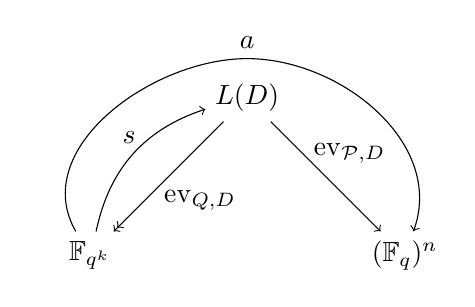
\begin{tikzpicture}
    \node (LD) at (2, 2) {$L(D)$};
    \node (Fqk) at (0, 0) {$\mathbb{F}_{q^k}$};
    \node (Fqn) at (4, 0) {$(\mathbb{F}_{q})^n$};
    \draw[->>] (LD) to (Fqk);
    \draw[->] (LD) to (Fqn);
    \draw[->] (Fqk) to[bend left] (LD);
    \node (s) at (0.5, 1.5) {$s$};
    \node (evQ) at (1.4, .7) {$\ev_{Q, D}$};
    \node (evP) at (3.3, 1.3) {$\ev_{\Pcal, D}$};
    \draw[->] (Fqk) to[out=120,in=180](2, 2.5) to[out=0, in=70] (Fqn);
    \node (a) at (2, 2.7) {$a$};
  \end{tikzpicture}
  \end{center}
Observe that $a$ is linear, so we can write
\[ a(x) = (\varphi_1(x), \dots, \varphi_n(x)) \]
where $\varphi_i:\mathbb{F}_{q^k}\to\mathbb{F}_{q}$ is a linear form, namely $\varphi_i(x)=f_x(P_i)$.



  Similarly, since the map $\ev_{\Pcal, tD}$ is injective, it admits a left inverse, \ie a linear
  map $r: (\mathbb{F}_{q})^n \to L(tD)$
  such that $r\circ\ev_{\Pcal, tD} = \Id_{L(tD)}$.
We also let $b: (\mathbb{F}_{q})^n \to \mathbb{F}_{q^k}$
  be the composite map $b = \ev_{Q, tD}\circ r$.   The situation is sumed up in the
  following drawing.
  \begin{center}
  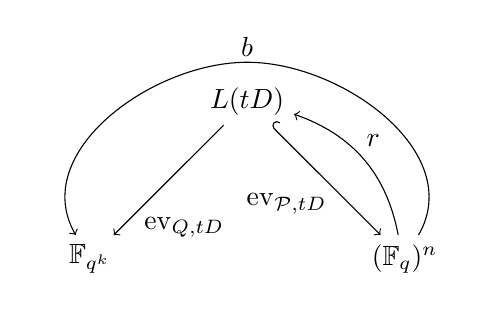
\begin{tikzpicture}
    \node (LtD) at (2, 2) {$L(tD)$};
    \node (Fqk) at (0, 0) {$\mathbb{F}_{q^k}$};
    \node (Fqn) at (4, 0) {$(\mathbb{F}_{q})^n$};
    \draw[right hook->] (LtD) to (Fqn);
    \draw[->] (LtD) to (Fqk);
    \draw[->] (Fqn) to[bend right] (LtD);
    \node (evP) at (2.5, .7) {$\ev_{\Pcal, tD}$};
    \node (s) at (3.6, 1.5) {$r$};
    \node (evQ) at (1.2, .4) {$\ev_{Q, tD}$};
    \draw[->] (Fqn) to[out=60,in=0](2, 2.5) to[out=180, in=120] (Fqk);
    \node (d) at (2, 2.7) {$b$};
  \end{tikzpicture}
\end{center}
The map $b$ is linear, so there are $b_1, \dots, b_n$ in
  $\mathbb{F}_{q^k}$ such that, for all $y=(y_1, \dots, y_n)\in(\mathbb{F}_{q})^n$,
  \[
    b(y) = \sum_{i=1}^n y_i b_i.
  \]

Now for $x,\dots,x_t\in\mathbb{F}_{q^k}$, let
  \[
    p = (p_1,\dots,p_n) = ((\prod_{j=1}^tf_{x_j})(P_1), \dots, (\prod_{j=1}^tf_{x_j})(P_n))
  \]
in $(\mathbb{F}_{q})^n$  be the coordinatewise product of the vectors $a(x_1)$, ..., $a(x_t)$.
Then
\[
  h = r(p)
\]
is an element of $L(tD)$ such that $h(P_i) = p_i = (\prod_{j=1}^tf_{x_j})(P_i)$ for all $i$.
Since the map $\ev_{\Pcal, tD}$ is injective, this forces
\[
  h = \prod_{j=1}^tf_{x_j}.
\]
Then, we have
\begin{equation*}
b(p) = \ev_{Q, tD}(r(p))
  = \ev_{Q, tD}(h)
  = h(Q)
  = \prod_{j=1}^t f_{x_j}(Q)
  = \prod_{j=1}^t x_j.
\end{equation*}
But we also have
\[
  b(p) = \sum_{i=1}^np_ib_i=\sum_{i=1}^n(\prod_{j=1}^tf_{x_j}(P_i))b_i=\sum_{i=1}^n(\prod_{j=1}^t\varphi_i(x_j))b_i
\]
and finally we get a symmetric formula for $m_t$:
\[
  \prod_{j=1}^t x_j = \sum_{i=1}^n(\prod_{j=1}^t\varphi_i(x_j))b_i.
\]
\end{proof}

\begin{prop}
\label{prop:numerical}
Let $F/\mathbb{F}_{q}$ be an algebraic function field of genus $g$.
Assume that $F$ admits a place $Q$ of degree $k$, and a set $\mathcal{S}$ of places of degree $1$ of cardinality
\[
  |\mathcal{S}|\geq (k+g-1)t+1.
\]
Then we have
\[ \musym_q(k,m_t)\leq kt+(g-1)(t-1). \]
\end{prop}
\begin{proof}
Set $n=kt+(g-1)(t-1)$. We will show that there are places $P_1,\dots,P_n$ in $\mathcal{S}$,
and a divisor $D$ on $F$, such that Proposition~\ref{prop:method} applies,
which gives $\musym_q(k,m_t)\leq n$ as desired.

Using e.g. \cite[Lemma~2.1]{Ballet99} we know $F$ admits a non-special divisor $R$ of degree $g-1$.
By the strong approximation theorem \cite[Thm.~1.6.5]{Stichtenoth09}
we can then find a divisor $D$ linearly equivalent to $R+Q$ and of support disjoint from $Q$ and $\mathcal{S}$.

Then $D-Q$ and $D$ are non-special, with $\ell(D-Q)=0$ and $\ell(D)=k$.
We thus find
\[
  \Ker(\ev_{Q, D}:L(D)\to\mathbb{F}_{q^k}) = L(D-Q) = 0,
\]
so $\ev_{Q, D}$ is injective, hence also surjective by equality of dimensions,
\ie the surjectivity condition~\ref{cond:1} in Proposition~\ref{prop:method} is satisfied.

Likewise, $tD$ is non-special, with $\deg(tD)=(k+g-1)t$ and $\ell(tD)=kt+(g-1)(t-1)$.
Then the evaluation map
\[
\begin{array}{cccc}
\ev_{\mathcal{S}, tD}: & L(tD) & \to & (\mathbb{F}_{q})^{|\mathcal{S}|}\\
  & h & \mapsto & (h(P))_{P\in\mathcal{S}}
\end{array}
\]
has kernel $L(tD-\sum_{P\in\mathcal{S}}P)=0$, because $\deg(tD-\sum_{P\in\mathcal{S}}P)=(k+g-1)t-|\mathcal{S}|<0$.
So $\ev_{\mathcal{S}, tD}$ is injective, with image of dimension $\dim\Img(\ev_{\mathcal{S}, tD})=\ell(tD)=n$.
Then we can find a subset $\Pcal=\{P_1,\dots,P_n\}\subset\mathcal{S}$ of cardinality $n$,
such that $\ev_{\Pcal, tD}: L(tD) \to (\mathbb{F}_{q})^n$ is an isomorphism,
and the injectivity condition~\ref{cond:2} in Proposition~\ref{prop:method} is also satisfied.
\end{proof}

\paragraph{Choice of the curves for $q$ a large enough square.}

\begin{prop}
\label{prop:asymptsquare}
Let $t$ be given, and assume $q$ is a square, $q\geq(t+2)^2$.
Then we have
\[
\Msym_{q,t}\leq(1+\epsilon_t(q))t
\]
with $\epsilon_t(q)=\frac{t-1}{\sqrt{q}-t-1}$.
\end{prop}
\begin{proof}
We know~\cite{STV92} that there exists a family of function fields
$F_i/\mathbb{F}_q$ of genus $g_i\to\infty$ such that
\begin{enumerate}[(i)]
  \item $\frac{g_{i+1}}{g_i}\to1$
  \item $N_i\sim (\sqrt q - 1)g_i$
\end{enumerate}
where $N_i = \Card\left\{ P\in\mathbb{P}_{F_i}\,|\,\deg P = 1 \right\}$
is the number of places of degree $1$ of $F_i$. We can also assume that the sequence
$g_i$ is increasing. 

For any $k$ let $i(k)$ be the smallest index such that
\[ N_{i(k)} \geq (k + g_{i(k)}-1)t +1. \]
Such an $i(k)$ always exists since by (ii) we have $N_i\sim (\sqrt q - 1)g_i$,
with $\sqrt q - 1>t$.

By definition we thus have
\[ N_{i(k)} \geq (k + g_{i(k)}-1)t +1 > (k + g_{i(k)-1}-1)t +1 > N_{i(k)-1}. \]
As $k\to\infty$ we have $i(k)\to\infty$, and by (i) we get $g_{i(k)}\sim g_{i(k)-1}$,
so by (ii) we also get $N_{i(k)}\sim N_{i(k)-1}$. This then gives
\[ \begin{split} N_{i(k)} &\sim (k + g_{i(k)}-1)t +1\\ &\sim (k + g_{i(k)})t \end{split} \]
while by (ii),
\[ N_{i(k)} \sim (\sqrt q - 1)g_{i(k)}. \]
From these two relations we deduce
\[ g_{i(k)} \sim \frac{t}{\sqrt{q}-1-t}k. \]
For $k$ large enough this implies in particular $2g_{i(k)} +1 \leq q^{(k-1)/2}(\sqrt q-1)$,
so $F_{i(k)}$ admits a place of degree $k$ by~\cite[Cor.~5.2.10]{Stichtenoth09}.

From this we are allowed to apply Proposition~\ref{prop:numerical} to $F_{i(k)}$, which gives
\[ \musym_q(k,m_t)\;\leq\; kt+(g_{i(k)}-1)(t-1)\;\sim\; kt+g_{i(k)}(t-1)\;\sim\; kt(1+\epsilon_t(q)) \]
as desired.
\end{proof}

\begin{cor}
\label{cor:asymptsquare}
For $q$ a square, $q\geq(t+3)^2$ we have
\[
\Mhyp_{q,t}\leq(1+\epsilon_{t+1}(q))(t+1),
\]
and in particular we have
\[ \Mtri_q\leq 3\left(1+\frac{2}{\sqrt{q}-4}\right) \]
for $q$ a square, $q\geq 25$.
\end{cor}

\paragraph{Conclusion for arbitrary $q$.}

\begin{lm}
\label{lemma:basechange}
Let $q$ be a prime power. Then for any integers $t,d,k$ we have
\[ \musym_q(k,m_t)\leq\musym_q(dk,m_t)\leq\musym_q(d,m_t)\musym_{q^d}(k,m_t). \]
\end{lm}
\begin{proof}
For the inequality on the left, there is nothing to prove if $\musym_q(dk,m_t)=\infty$.
So let us assume $m_t^{\mathbb{F}_{q^{dk}}/\mathbb{F}_{q}}$ admits a symmetric multiplication formula of length $n=\musym_q(dk,m_t)$, \ie
\[\forall x_1,\dots,x_t\in\mathbb{F}_{q^{dk}},\quad x_1\cdots x_t = \sum_{i=1}^{n}\varphi_i(x_1)\cdots\varphi_i(x_t)a_i \]
for linear forms $\varphi_i:\mathbb{F}_{q^{dk}}\to\mathbb{F}_{q}$ and elements $a_i\in\mathbb{F}_{q^{dk}}$.
Choose a linear projection
\[ p:\mathbb{F}_{q^{dk}}\to\mathbb{F}_{q^{k}} \]
left inverse for the inclusion $\mathbb{F}_{q^{k}}\subseteq\mathbb{F}_{q^{dk}}$.
Then we get
\[\forall x_1,\dots,x_t\in\mathbb{F}_{q^{k}},\quad x_1\cdots x_t = p(x_1,\dots,x_t) = \sum_{i=1}^{n}\varphi_i(x_1)\cdots\varphi_i(x_t)p(a_i) \]
which is a symmetric multiplication formula of length $n$ for $m_t^{\mathbb{F}_{q^{k}}/\mathbb{F}_{q}}$.

Likewise, for the inequality on the right, there is nothing to prove if $\musym_q(d,m_t)=\infty$ or $\musym_{q^d}(k,m_t)=\infty$.
So let us assume $m_t^{\mathbb{F}_{q^{d}}/\mathbb{F}_{q}}$ and $m_t^{\mathbb{F}_{q^{dk}}/\mathbb{F}_{q^{d}}}$ admit symmetric multiplication formulae of length $r=\musym_q(d,m_t)$ and $s=\musym_{q^d}(k,m_t)$ respectively, so
\vspace{-.5\baselineskip}

\[\forall y_1,\dots,y_t\in\mathbb{F}_{q^{d}},\quad y_1\cdots y_t = \sum_{u=1}^{r}\psi_u(y_1)\cdots\psi_u(y_t)b_u \]
\vspace{-1.5\baselineskip}

\[\forall z_1,\dots,z_t\in\mathbb{F}_{q^{dk}},\quad z_1\cdots z_t = \sum_{v=1}^{s}\chi_v(z_1)\cdots\chi_v(z_t)c_v \]
\vspace{-.5\baselineskip}

\noindent for linear forms $\psi_u:\mathbb{F}_{q^{d}}\to\mathbb{F}_{q}$, $\chi_v:\mathbb{F}_{q^{dk}}\to\mathbb{F}_{q^{d}}$ and elements $b_u\in\mathbb{F}_{q^{d}}$, $c_v\in\mathbb{F}_{q^{dk}}$.
Then setting $y_1=\chi_v(z_1)$, ..., $y_t=\chi_v(z_t)$ we find
\[\forall z_1,\dots,z_t\in\mathbb{F}_{q^{dk}},\quad z_1\cdots z_t = \sum_{v=1}^{s}\sum_{u=1}^{r}(\psi_u\circ\chi_v)(z_1)\cdots(\psi_u\circ\chi_v)(z_t)\cdot(b_uc_v) \]
which is a symmetric multiplication formula of length $rs$ for $m_t^{\mathbb{F}_{q^{dk}}/\mathbb{F}_{q}}$.
\end{proof}


\begin{thm}
Let $t\geq2$ be an integer and $q$ a prime power.
If $q<t$, then $\musym_q(k,m_t)=\infty$ for all $k\geq2$.

On the other hand, if $q\geq t$,
then $\musym_q(k,m_t)$ grows at most linearly with $k$, \ie we have
\[
\Msym_{q,t}\leq C_t(q)
\]
for some real constant $C_t(q)<\infty$.
\end{thm}
\begin{proof}
If $q<t$ and $k\geq2$, then $\musym_q(k,m_t)=\infty$ follows from Theorem~\ref{th:criterion}.

On the other hand, for $q\geq t$, we have $\musym_q(d,m_t)<\infty$ for any integer $d$.
Choose $d$ such that $q^d$ is a square, $q^d\geq(t+2)^2$.
Then Proposition~\ref{prop:asymptsquare} shows $\musym_{q^d}(k,m_t)$ grows linearly with $k$.
The Theorem then follows thanks to Lemma~\ref{lemma:basechange}, with $C_t(q)=\musym_q(d,m_t)(1+\epsilon_t(q^d))t$.
\end{proof}
\begin{cor}
For $q\geq t+1$ we have
\[
\Mhyp_{q,t}\leq C_{t+1}(q)
\]
and in particular for $q\geq 3$ we have
\[
\Mtri_q\leq C_{3}(q).
\]
\end{cor}

\paragraph{Further remarks and possible improvements.}
\begin{enumerate}
\item When $q\geq4$ is not divisible by $3$, \cite[Thm.~2]{SL84} gives $\mutri_q(k)\leq 4\musym_q(k)$.
On the other hand, \cite{CC88} shows that $\musym_q(k)$ grows linearly with $k$ (the result is stated for $\mu_q(k)$,
but it is easily seen that the proof works for $\musym_q(k)$). Joint together, these results show that $\mutri_q(k)$ grows linearly with $k$
when $q\geq4$ is not divisible by $3$. One advantage of our method is that it works for all $q\geq3$.
Moreover it gives sharper bounds. For instance, when $q$ is a square and large enough, joining \cite[Thm.~2]{SL84} with the best asymptotic upper bound known on $\musym_q(k)$ \cite[Thm.~6.4]{Randriam12} gives $\Mtri_q\leq 8\left(1+\frac{1}{\sqrt{q}-2}\right)$,
which is not as good as $\Mtri_q\leq 3\left(1+\frac{2}{\sqrt{q}-4}\right)$ from Corollary~\ref{cor:asymptsquare}.
\item \emph{Open question}: Lemma~\ref{lm:hyp<sym+1} reduces (upper) bounds on $\muhyp(m_t)$ to bounds on $\musym(m_{t+1})$,
and in particular it reduces bounds on $\Mtri_q$ to bounds on $\Mhyp_{q,3}$, which does not seem optimal.
Indeed we know no example where the inequality $\musym_q(k)\leq\mutri_q(k)$ is strict.
So, for instance for $q$ square, $q\to\infty$, our method gives $\Mtri_q\leq 3(1+o(1))$,
but one could ask whether it is possible to get a bound of the form $\Mtri_q\leq 2(1+o(1))$,
as given by \cite[Thm.~6.4]{Randriam12} for $\Msym_q$.
\item \emph{Open question}: The condition $|\mathcal{S}|\geq (k+g-1)t+1$ in Proposition~\ref{prop:numerical}
does not seem optimal since in the end we do evaluation-interpolation at only $kt+(g-1)(t-1)$ places.
If one could relax this condition to $|\mathcal{S}|\geq kt+(g-1)(t-1)$, this would improve Proposition~\ref{prop:asymptsquare}
to $\Msym_{q,t}\leq(1+\epsilon'_t(q))t$ for $q$ square, $q\geq(t+1)^2$,
with $\epsilon'_t(q)=\frac{t-1}{\sqrt{q}-t}$.
For $t=2$ this is done in \cite{Randriam12,Randriam19} using techniques from \cite{Randriam13}.
However, as observed at the end of \cite{Randriam13}, a generalization to $t\geq3$ would require new arguments.
\item Lemma~\ref{lemma:basechange}, which generalizes \cite[Lemma~1.2]{STV92}, is clearly not optimal.
When deriving upper bounds on $\musym_q(k,m_t)$ for non-square $q$, it might be better to use evaluation-interpolation
at places of higher degree, as first introduced in~\cite{BR04}, and further developped e.g. in~\cite{CCXY12,Randriam12}.
To do this in an optimal way one needs function fields $F_i$ defined over $\mathbb{F}_q$,
of genus $g_i\to\infty$, with $\frac{g_{i+1}}{g_i}\to 1$ and $N_i^{(d)}\sim\frac{q^{d/2}-1}{d}g_i$
where $N_i^{(d)}$ is the number of places of degree $d$ in $F_i$, for a convenient $d$.
This improves the bound on $\Msym_{q,t}$ by a factor $\frac{1}{d}$.
The existence of these function fields was first claimed in \cite{CCXY12}, but unfortunately with an incorrect proof.
A corrected construction, based on Drinfeld modular curves, will be found in \cite{BBRR20+}.
\item All our bounds for multiplication in extension fields also hold for truncated polynomials.
For instance we have $\hat{M}^{\textrm{sym}}_{q,t}\leq(1+\epsilon_t(q))t$ for $q$ square, $q\geq(t+2)^2$,
and $\hat{M}^{\textrm{sym}}_{q,t}\leq C_t(q)$ for all $q\geq t$.
This requires only minor changes in our constructions.
In Proposition~\ref{prop:method}, instead of evaluation at a place $Q$ of degree~$k$, one uses evaluation at order $k$
at an extra place $P_0$ of degree~$1$.
Likewise in Proposition~\ref{prop:numerical}, one needs one more place of degree~$1$, but one does not need $Q$
(then the proof of Proposition~\ref{prop:asymptsquare} is slightly simplified since one does not need to invoke \cite[Cor.~5.2.10]{Stichtenoth09} anymore).
\end{enumerate}

\small
\bibliographystyle{plain}
\bibliography{erou}

\end{document}
